\section{椭圆}

本节要点:
\begin{itemize}
    \item 掌握椭圆的概念;
    \item 从代数角度掌握椭圆的几何性质。
\end{itemize}

%============================================================
\subsection{椭圆及其标准方程}

\begin{definition}[椭圆]
设二维平面中有两个定点$F_1,F_2$,若平面上的点和$F_1,F_2$的距离之和都是$r>0$,则称这些点组成的集合为{\bf 椭圆},常用$E$表示,即:
\[
E:=\left\{ P \middle| \left| \overrightarrow{F_1P} \right|+\left| \overrightarrow{F_2P} \right|=r \right\}
\]
其中,$F_1,F_2$称为{\bf 焦点},$\left| \overrightarrow{F_1F_2} \right|$称为{\bf 焦距}。若令$F_1=\left( -c,0 \right) ,F_2=\left( c,0 \right) $,则椭圆可以表示为下列的{\bf 标准方程}:
\[
\frac{x^2}{a^2}+\frac{y^2}{b^2}=1
\]
其中$a,b,c$满足$a^2-b^2=c^2$。
\end{definition}

\begin{figure}[h]
\centering
\begin{tikzpicture}[line join=round, scale=0.4]
\pgfmathparse{0.6/0.4}
\mydrawxy{-7}{7}{-5}{5}
\coordinate[label=below left:{$O$}]   (O)  at (0,0);
\coordinate[label=below:     {$F_1$}] (F1) at (-4,0);
\coordinate[label=below:     {$F_2$}] (F2) at (4,0);
\coordinate[label=above:     {$P$}]   (P)  at (0,3);
\coordinate[label=right:     {$Q$}]   (Q)  at (5,0);
\draw[thick] (0,0) ellipse (5 and 3);
\fill (F1) circle (\pgfmathresult mm);
\fill (F2) circle (\pgfmathresult mm);
\draw (F1)--(P)--(F2);
\coordinate[label=above right:{$a$}] (a) at ($(P)!0.5!(F2)$);
\coordinate[label=left:       {$b$}] (b) at ($(P)!0.5!(0,0)$);
\coordinate[label=below:      {$c$}] (c) at ($(0,0)!0.5!(F2)$);
\end{tikzpicture}
\end{figure}

\begin{tcolorbox}
详细阅读课本关于椭圆标准方程的推导过程,体会两次平方的意义。详细阅读例2、例3、例6,可以认为是椭圆的另外三种定义。
\end{tcolorbox}

%============================================================
\subsection{椭圆的简单几何性质}

设有如下椭圆,我们称:
\begin{itemize}
    \item $O,A_1,A_2,B_1,B_2$:一个{\bf 中心}和四个{\bf 顶点};
    \item $A_1A_2=2a$:{\bf 长轴};
    \item $B_1B_2=2b$:{\bf 短轴};
    \item $F_1F_2=2c$:{\bf 焦距};
    \item $e=\frac{c}{a}=\cos \theta \in \left[ 0,1 \right) $:{\bf 离心率},$e$越大椭圆越扁平,$e=0$时退化为圆,$e\rightarrow 1$时变成两条平行线$y=\pm b$。
\end{itemize}

\begin{figure}[h]
\centering
\begin{minipage}{.49\textwidth}
\centering
\begin{tikzpicture}[line join=round, scale=0.3]
\mydrawxy{-7}{7}{-5}{5}
\coordinate[label=below left: {$O$}]   (O)  at (0,0);
\coordinate[label=above left: {$A_1$}] (A1) at (-5,0);
\coordinate[label=above right:{$A_2$}] (A2) at (5,0);
\coordinate[label=above left: {$B_1$}] (B1) at (0,3);
\coordinate[label=below left: {$B_2$}] (B2) at (0,-3);
\draw[thick] (0,0) ellipse (5 and 3);
\coordinate[label=below:{$a$}] (a) at ($(O)!0.5!(A2)-(0,0.5)$);
\coordinate[label=left: {$b$}] (b) at ($(O)!0.5!(B1)-(0.5,0)$);
\draw[decorate,decoration={calligraphic brace,raise=0cm,aspect=0.5,amplitude=0.2cm},thick] (A2)--(O);
\draw[decorate,decoration={calligraphic brace,raise=0cm,aspect=0.5,amplitude=0.2cm},thick] (O)--(B1);
\end{tikzpicture}
\end{minipage}
\begin{minipage}{.49\textwidth}
\centering
\begin{tikzpicture}[line join=round, scale=0.3]
\pgfmathparse{0.6/0.3}
\mydrawxy{-7}{7}{-5}{5}
\coordinate[label=below left:{$O$}]   (O)  at (0,0);
\coordinate[label=below:     {$F_1$}] (F1) at (-4,0);
\coordinate[label=below:     {$F_2$}] (F2) at (4,0);
\coordinate[label=above left:{$P$}]   (P)  at (0,3);
\coordinate[label=above right:{$Q$}]   (Q)  at (5,0);
\draw[thick] (0,0) ellipse (5 and 3);
\fill (F1) circle (\pgfmathresult mm);
\fill (F2) circle (\pgfmathresult mm);
\draw (F1)--(P)--(F2);
\coordinate[label=above right:{$a$}] (a) at ($(P)!0.5!(F2)$);
\coordinate[label=left:       {$b$}] (b) at ($(P)!0.5!(0,0)$);
\coordinate[label=below:      {$c$}] (c) at ($(0,0)!0.5!(F2)$);
\pic["$\theta $",draw,angle radius=0.5cm,angle eccentricity=1.5] {angle=P--F2--O};
\end{tikzpicture}
\end{minipage}
\end{figure}

%============================================================
\subsection{拓展讨论:坐标系变换}

\begin{tcolorbox}
对课本例2深入讨论。
\end{tcolorbox}

椭圆可以通过圆的拉伸获得,如下左图,圆方程为$x^2+y^2=2^2$:

\begin{figure}[h]
\centering
\begin{minipage}{.39\textwidth}
\centering
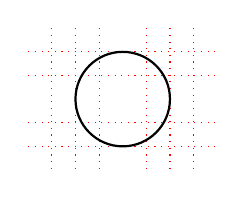
\begin{tikzpicture}[line join=round, scale=0.3]
\mydrawxy{-4}{4}{-3}{3}
\foreach \y in {-2,-1,1,2}      {\draw[dotted,red] (-4,\y)--(4,\y);}
\foreach \x in {-3,-2,-1,1,2,3} {\draw[dotted,red] (\x,3)--(\x,-3);}
\draw[thick] (0,0) circle(2);
\end{tikzpicture}
\end{minipage}
\begin{minipage}{.59\textwidth}
\centering
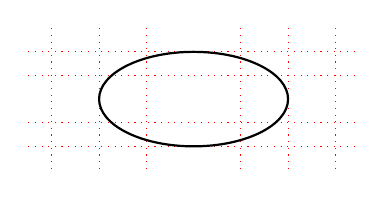
\begin{tikzpicture}[line join=round, scale=0.3]
\mydrawxy{-7}{7}{-3}{3}
\foreach \y in {-2,-1,1,2}      {\draw[dotted,red] (-7,\y)--(7,\y);}
\foreach \x in {-6,-4,-2,2,4,6} {\draw[dotted,red] (\x,3)--(\x,-3);}
\draw[thick] (0,0) ellipse (4 and 2);
\end{tikzpicture}
\end{minipage}
\end{figure}

我们进行坐标变换,将{\it x}轴拉长一倍,如上右图:
\[
\begin{cases}
	u=2x\\
	v=y\\
\end{cases}\Rightarrow \quad \begin{cases}
	x=0.5u\\
	y=v\\
\end{cases}
\]
则有:
\[
\frac{u^2}{4^2}+\frac{v^2}{2^2}=1
\]
可见,将坐标轴拉伸就可将圆变成椭圆,反之,将坐标轴压缩就可将椭圆变成圆。

%============================================================
\subsection{拓展讨论:斜率之积}

\begin{tcolorbox}
对课本例3深入讨论。
\end{tcolorbox}

设椭圆$E$及椭圆上一点$P$,如下左图,则$PA_1,PA_2$的斜率之积有:
\begin{align*}
&\because \frac{x^2}{a^2}+\frac{y^2}{b^2}=1 \\
&\therefore k_{PA_1}k_{PA_2}=\frac{y_P}{x_P+a}\cdot \frac{y_P}{x_P-a}=\frac{b^2\left( 1-\frac{{x_P}^2}{a^2} \right)}{{x_P}^2-a^2}=-\frac{b^2}{a^2}=-\tan ^2\theta
\end{align*}
特别地,当$a=b$时,$k_{PA_1}k_{PA_2}=-1$即$PA_1\bot PA_2$,此时椭圆退化为圆,如下右图。

\begin{figure}[h]
\centering
\begin{minipage}{.59\textwidth}
\centering
\begin{tikzpicture}[line join=round, scale=1]
\mydrawxy{-2}{2}{-1.2}{1.2}
\draw[thick] (0,0) ellipse (1.5 and 1);
\coordinate[label=left: {$A_1$}] (A1) at (-1.5,0);
\coordinate[label=right:{$A_2$}] (A2) at (1.5,0);
\coordinate[label=above:{$P$}]   (P)  at (1,0.745);
\coordinate[label=below:{$a$}] (a) at ($(0,0)!0.5!(A2)$);
\coordinate[label=left: {$b$}] (b) at ($(0,0)!0.5!(0,1)$);
\draw (A1)--(P)--(A2);
\end{tikzpicture}
\end{minipage}
\begin{minipage}{.39\textwidth}
\centering
\begin{tikzpicture}[line join=round, scale=1]
\mydrawxy{-2}{2}{-1.2}{1.2}
\draw[thick] (0,0) circle(1);
\coordinate[label=left: {$A_1$}] (A1) at (-1,0);
\coordinate[label=right:{$A_2$}] (A2) at (1,0);
\coordinate[label=above:{$P$}]   (P)  at (0.707,0.707);
\coordinate[label=below:{$a=b$}] (a) at ($(0,0)!0.5!(A2)$);
\coordinate[label=left: {$b$}]   (b) at ($(0,0)!0.5!(0,1)$);
\draw (A1)--(P)--(A2);
\end{tikzpicture}
\end{minipage}
\end{figure}

可见:
\begin{itemize}
    \item $k_1k_2\in \left( -\infty ,-1 \right) $:长条形椭圆;
    \item $k_1k_2=-1$:圆;
    \item $k_1k_2\in \left( -1,0 \right) $:扁宽形椭圆。
\end{itemize}

%============================================================
\subsection{拓展讨论:两个焦点}

\begin{tcolorbox}
对课本例5深入讨论。
\end{tcolorbox}

例5说明了从任意一个焦点出发的光线都能聚焦到另一个焦点,证明这点需要微积分的知识,略。但我们可以思考,当两个焦点重合的时候,从焦点出发的任意光线都能返回到焦点,这是一个圆,而且圆的半径总是垂直于切线。

\begin{figure}[h]
\centering
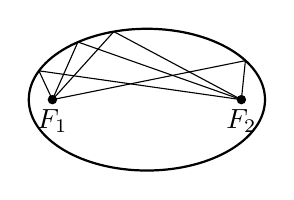
\begin{tikzpicture}[line join=round, scale=0.3]
\pgfmathparse{0.6/0.3}
\mydrawxy{-6}{6}{-3.5}{3.5}
\draw[thick] (0,0) ellipse (5 and 3);
\coordinate[label=below:{$F_1$}] (F1) at (-4,0);
\coordinate[label=below:{$F_2$}] (F2) at (4,0);
\fill (F1) circle (\pgfmathresult mm);
\fill (F2) circle (\pgfmathresult mm);
\coordinate (A) at (-4.57,1.22);
\coordinate (B) at (-2.92,2.44);
\coordinate (C) at (-1.4,2.88);
\coordinate (D) at (4.17,1.65);
\foreach \p in {A,B,C,D} {\draw (F1)--(\p)--(F2);}
\end{tikzpicture}
\end{figure}

有些音乐厅就设计成椭圆,乐队位于一个焦点附近,VIP位于另一个焦点附近,使得VIP在听觉上能位于乐队中。

%============================================================
\subsection{拓展讨论:动点距离直线}

\begin{tcolorbox}
对课本例6深入讨论。
\end{tcolorbox}

我们考察,对于任意一个椭圆$E$,是否必有垂直坐标轴的直线$x=x_0$,且椭圆上的点$P$距离焦点和直线的比是定值$k$。

\begin{figure}[h]
\centering
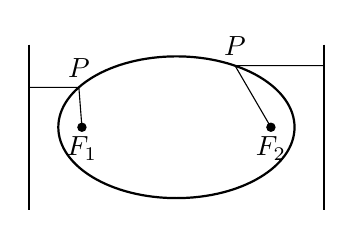
\begin{tikzpicture}[line join=round, scale=0.3]
\pgfmathparse{0.6/0.3}
\mydrawxy{-7}{7}{-3.5}{3.5}
\draw[thick] (0,0) ellipse (5 and 3);
\coordinate[label=below:{$F_1$}] (F1) at (-4,0);
\coordinate[label=below:{$F_2$}] (F2) at (4,0);
\coordinate[label=above:{$P$}]   (P1) at (-4.13,1.69);
\coordinate[label=above:{$P$}]   (P2) at (2.48,2.61);
\fill (F1) circle (\pgfmathresult mm);
\fill (F2) circle (\pgfmathresult mm);
\draw[thick] (-6.25,3.5)--(-6.25,-3.5) (6.25,3.5)--(6.25,-3.5);
\draw (F1)--(P1)--(-6.25,1.69) (F2)--(P2)--(6.25,2.61);
\end{tikzpicture}
\end{figure}

距离焦点和直线的比:
\begin{align*}
&\frac{x^2}{a^2}+\frac{y^2}{b^2}=1 \\
&k=\frac{\sqrt{\left( x\pm c \right) ^2+y^2}}{\left| x-x_0 \right|}\Rightarrow k^2\left( x-x_0 \right) ^2=\left( x\pm c \right) ^2+y^2
\end{align*}
化简后得:
\[
\left( 1-k^2-\frac{b^2}{a^2} \right) x^2+2\left( k^2x_0\pm c \right) x+\left( a^2-k^2{x_0}^2 \right) =0
\]
若要对所有$x$都成立,必须:
\[
\begin{cases}
	1-k^2-\frac{b^2}{a^2}=0\\
	k^2x_0\pm c=0\\
	a^2-k^2{x_0}^2=0\\
\end{cases}\Rightarrow \quad \begin{cases}
	k=\frac{c}{a}\in \left( 0,1 \right) \\
	x_0=\mp \frac{a^2}{c}\\
\end{cases}
\]
不难发现特点:
\begin{itemize}
    \item 对于左焦点有左边的直线$x=-\frac{a^2}{c}$,对于右焦点有右边的直线$x=\frac{a^2}{c}$,且两条直线一定在椭圆外侧;
    \item 动点距离焦点更近;
    \item 当$c=0$时椭圆退化为圆,且$x_0=\pm \infty ,k=0$,表示直线为无穷远处,自行脑补。
\end{itemize}

%============================================================
\subsection{拓展讨论:椭圆的一般方程}

教材中对于直线和圆都有一般形式的方程,为什么椭圆就没有?我们来推导一下椭圆方程的一般形式,从最一般的二次曲线开始,如下:
\[
Ax^2+By^2+Cxy+Dx+Ey+F=0
\]
$A,D$和$B,E$可以凑出$x,y$的平方项,一方面只影响$F$,另一方面$x,y$的平方项可以通过坐标平移解决,所以我们可以之分析如下形式:
\[
Ax^2+By^2+Cxy+F=0
\]
易得该方程对应的曲线关于原点对称。

我们先考察另一个问题,将椭圆绕中心点沿顺时针转$\alpha $后方程是什么样子的。设椭圆如下:
\[
\frac{x^2}{a^2}+\frac{y^2}{b^2}=1
\]
转换为极坐标形式:
\[
\frac{\left( r\cos \theta \right) ^2}{a^2}+\frac{\left( r\sin \theta \right) ^2}{b^2}=1
\]
将椭圆绕中心点沿顺时针转$\alpha $:
\[
\frac{\left[ r\cos \left( \theta -\alpha \right) \right] ^2}{a^2}+\frac{\left[ r\sin \left( \theta -\alpha \right) \right] ^2}{b^2}=1 \qquad \alpha \in \left[ 0,\pi \right)
\]
注意我们这里是顺时针转动图形,相当于逆时针转动坐标系,所以是$-\alpha $而不是$+\alpha $,展开后:
\begin{align*}
&\left( b^2\cos ^2\alpha +a^2\sin ^2\alpha \right) x^2+\left( b^2\sin ^2\alpha +a^2\cos ^2\alpha \right) y^2-c^2\sin 2\alpha xy=a^2b^2 \\
&Ax^2+By^2+Cxy+F=0 \\
&\begin{cases}
	A=b^2\cos ^2\alpha +a^2\sin ^2\alpha =b^2+\frac{c^2}{2}\left( 1-\cos 2\alpha \right)\\
	B=b^2\sin ^2\alpha +a^2\cos ^2\alpha =b^2+\frac{c^2}{2}\left( 1+\cos 2\alpha \right)\\
	C=-c^2\sin 2\alpha\\
	F=-a^2b^2\\
\end{cases}
\end{align*}
不难发现:
\begin{itemize}
    \item $F<0$,若$F>0$则曲线不存在,若$F=0$则有可能是一点有可能是直线;
    \item $A,B>0$,否则变成双曲线,且有$A+B=a^2+b^2$,当$A=B$时$\alpha =\pi /4$或$3\pi /4$;
    \item $A,F>0$共同决定了椭圆和{\it x}轴的交点,$B,F>0$共同决定了椭圆和{\it y}轴的交点。
\end{itemize}
特别地,当$\alpha =\pi /4$时,方程为在圆的基础上加一个$xy$项,如下:
\[
\left( a^2+b^2 \right) x^2+\left( a^2+b^2 \right) y^2-2c^2xy=2a^2b^2
\]
当$\alpha =\pi /2$时,表现为长短轴互换,如下:
\[
a^2x^2+b^2y^2=a^2b^2
\]

%============================================================
\subsection{习题}

\begin{example}[复习巩固6,难度:$\star $]
如图,圆$O$的半径为定长$r$,$A$是圆$O$内一个定点,$P$是圆$O$上任意一点。线段$AP$的垂直平分线$l$和半径$OP$相交于点$Q$,当点$P$在圆上运动时,点$Q$的轨迹是什么?为什么?
\end{example}

\begin{figure}[h]
\centering
\begin{tikzpicture}[line join=round, scale=1.25]
\draw[thick] (0,0) circle(1);
\coordinate[label=below:      {$O$}] (O) at (0,0);
\coordinate[label=above:      {$P$}] (P) at (0.34,0.94);
\coordinate[label=right:      {$A$}] (A) at (0.76,0.33);
\coordinate[label=above right:{$B$}] (B) at ($(P)!0.5!(A)$);
\coordinate[label=left:       {$Q$}] (Q) at ($(O)!0.35!(P)$);
\draw (O)--(P)--(A) ($(Q)!-3.0!($(P)!(Q)!(A)$)$)--($(Q)!2.0!($(P)!(Q)!(A)$)$);
\draw[red] (Q)--(A);
\end{tikzpicture}
\end{figure}

解:

连接$QA$,有:
\[
QO+QA=QO+QP=r
\]

\begin{tcolorbox}
仔细观察图形,本题没有难度。不要盲目建立坐标系,椭圆的中心未知。
\end{tcolorbox}

~

\begin{example}[拓广探索14,难度:$\star $]
已知椭圆$\frac{x^2}{4}+\frac{y^2}{9}=1$,一组平行直线的斜率是$\frac{3}{2}$。
\begin{enumerate}
    \item 这组直线何时与椭圆有两个公共点?
    \item 当它们与椭圆有两个公共点时,证明这些直线被椭圆截得的线段的中点在同一条直线上。
\end{enumerate}
\end{example}

解:

(1)略。

(2)一般的做法是假设直线$y=\frac{3}{2}x+c$,带入椭圆求交点:
\begin{align*}
&18x^2+12cx+4c^2-36=0 \\
&x_{1,2}=\frac{-12c\pm \sqrt{144c^2-4\cdot 18\cdot \left( 4c^2-36 \right)}}{36}
\end{align*}
得到线段中点:
\[
\begin{cases}
	x_0=-\frac{1}{3}c\\
	y_0=\frac{1}{2}\\
\end{cases}
\]
是一个参数方程,就是一条过原点,斜率是$-3/2$的直线。

但是,理解了坐标系变换,可以先压缩{\it xy}两个轴,使得椭圆变成一个标注圆,此时,这一组平行线将变成:
\[
y=x+c
\]
不难发现割线的中点是直线$y=-x$,最后通过拉伸{\it xy}两个轴变回来,略。

\begin{tcolorbox}
本题没有难度,但从坐标系变换的角度分析,还是有点意思的。
\end{tcolorbox}




